\begin{enumerate}
	\item Exercício
	
	\begin{figure}[H]
		\centering
		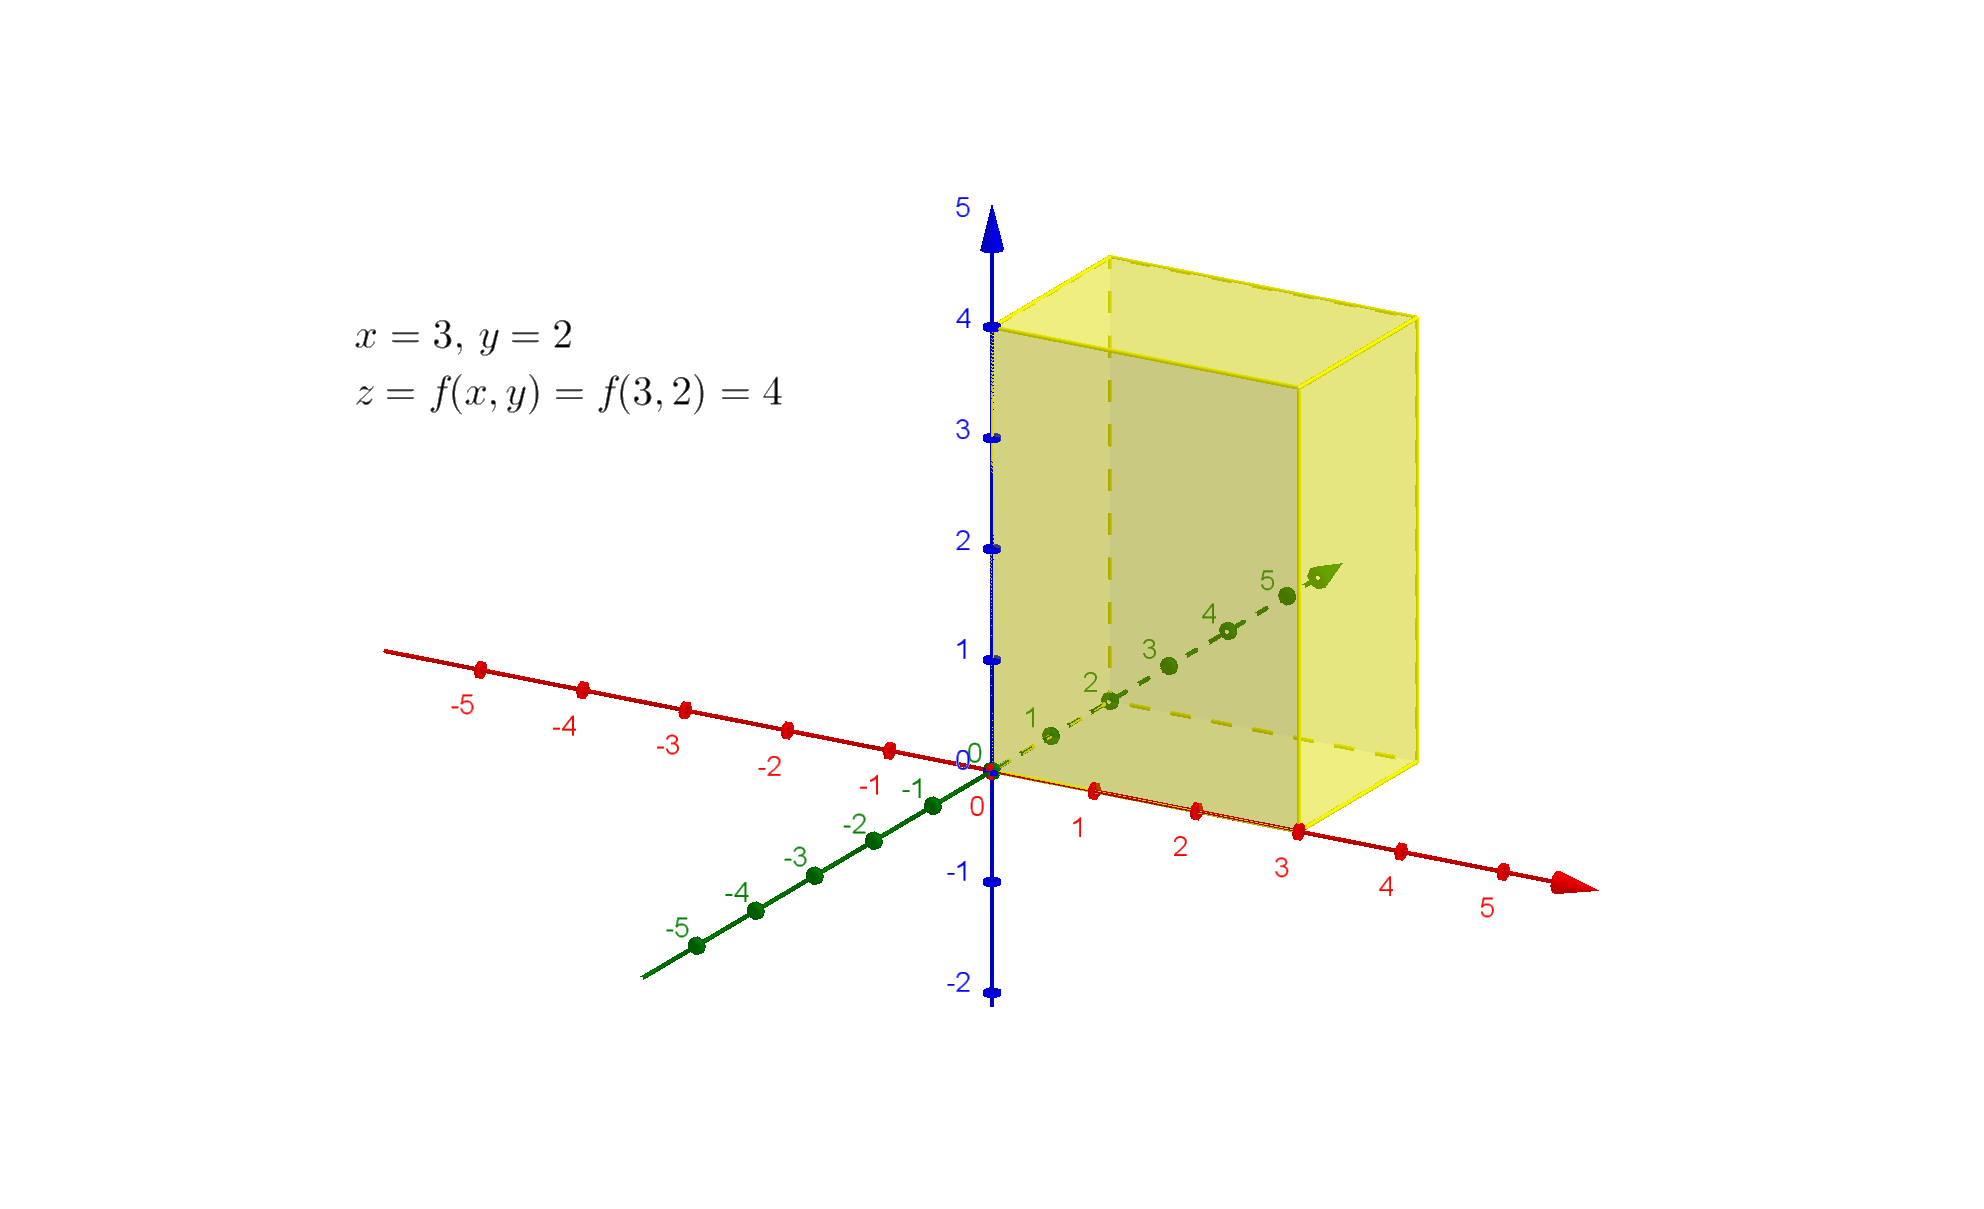
\includegraphics[width=\textwidth]{v01_a03_e01.png}
		\caption{Integrais duplas - Aula 3 - Exercício I}
		\label{v01_a03_e01}
	\end{figure}
	
	$z = 4;\; dz = dx dy$\newline\newline
	$v = \integral_0^3 \integral_0^2 z\, dz = \integral_0^3 \integral_0^2 4\, dy dx = 4\integral_0^3 dx \integral_0^2 dy = 4\integral_0^3 dx\, [y]_0^2 = 4\integral_0^3 dx\, [2 - 0] = 8\integral_0^3 dx = 8[x]_0^3 = 8[3 - 0] = 8 \cdot 3 = 24$\newline
	
	\item Exercício
	
	$R = [0, 3] \times [0,4]\\
	\integral \integral_R (8 - 2y) da$
	
	\begin{figure}[H]
		\centering
		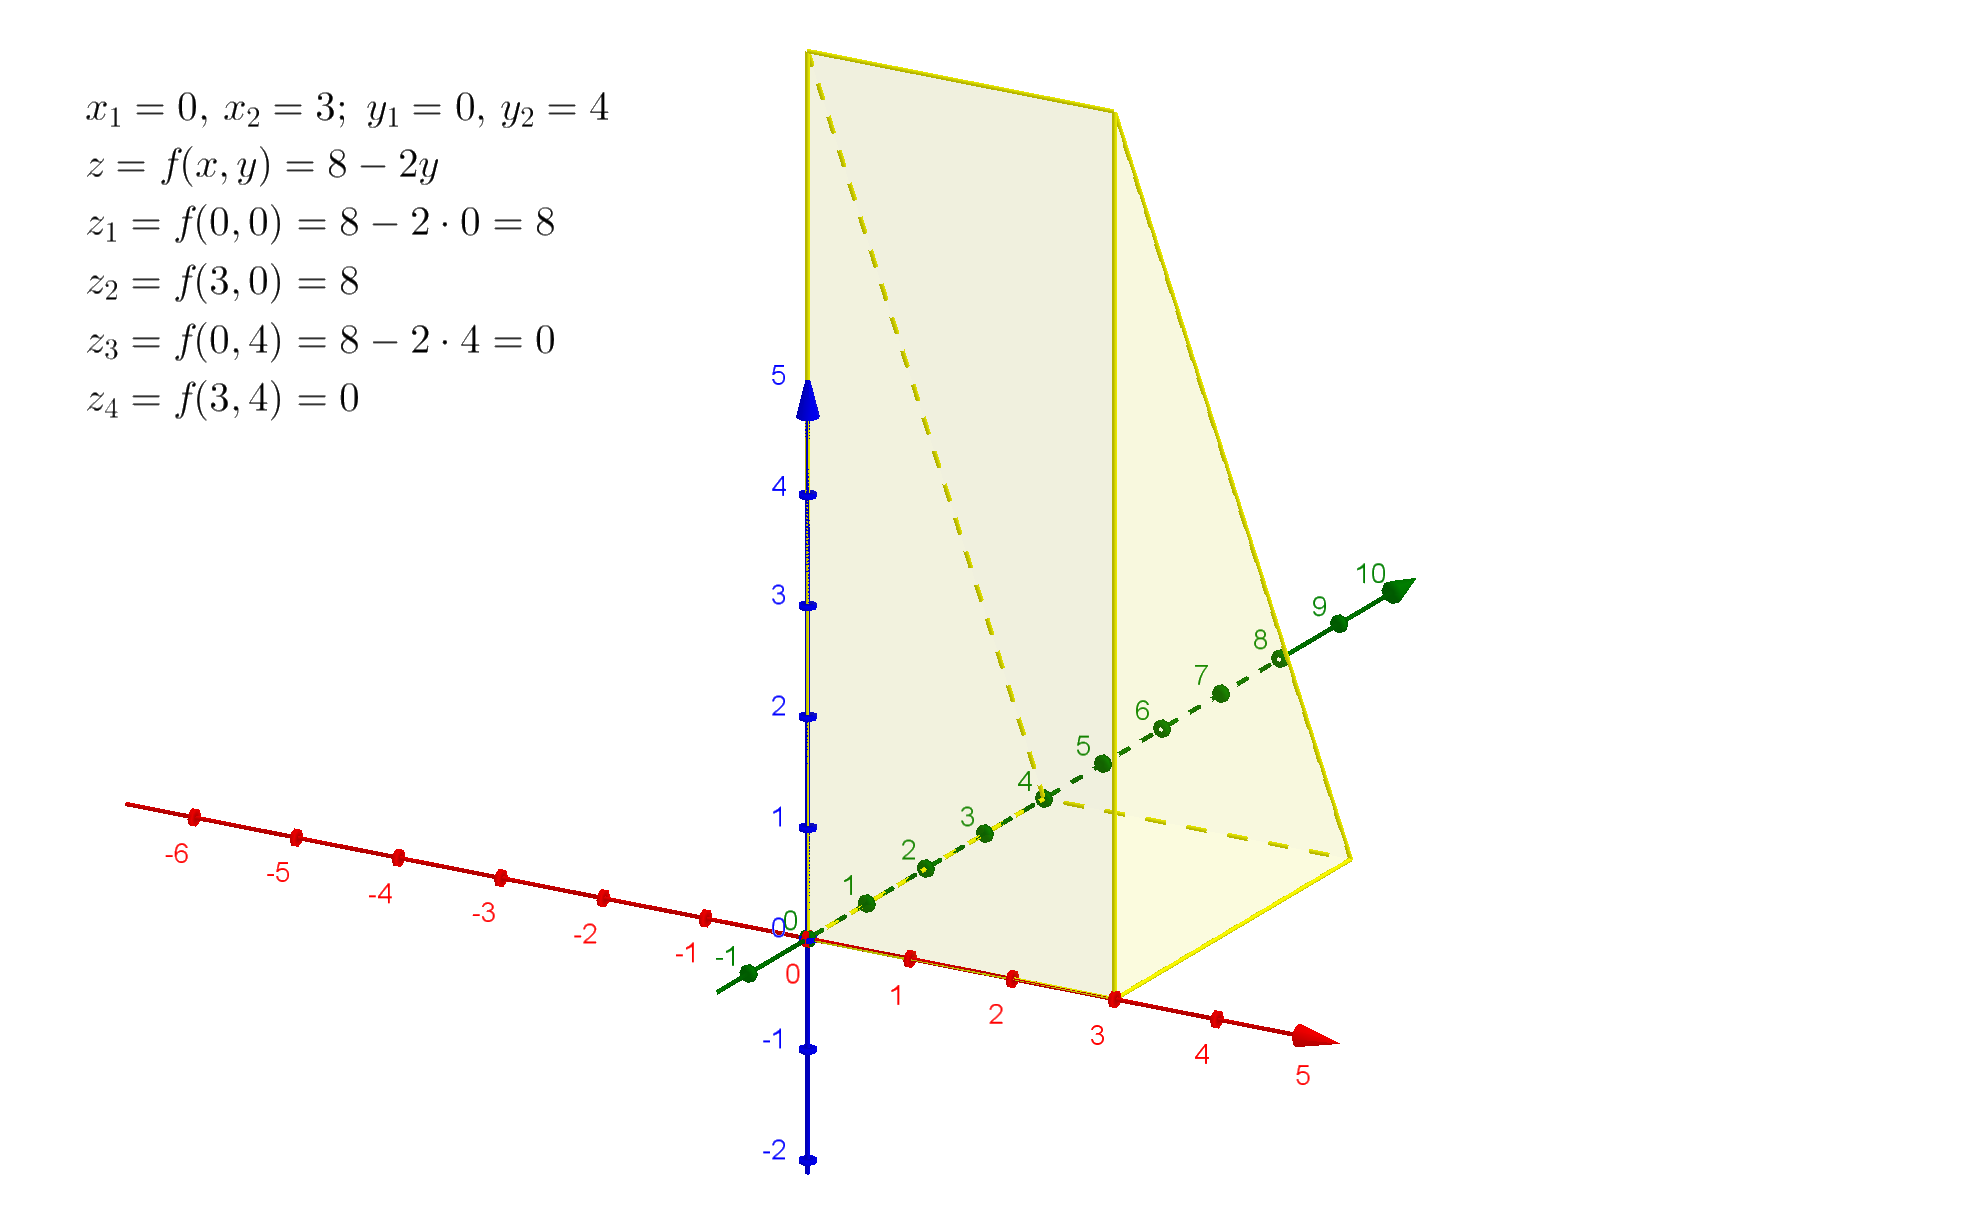
\includegraphics[width=\textwidth]{v01_a03_e02.png}
		\caption{Integrais duplas - Aula 3 - Exercício II}
		\label{v01_a03_e02}
	\end{figure}	
	
	$z = 8 - 2y;\; da = dz = dx dy$\newline\newline
	$v = \integral_0^3 \integral_0^4 z\,dz = \integral_0^3 \integral_0^4(8 - 2y)dx dy = \integral_0^3 dx \integral_0^4(8 - 2y) dy = \integral_0^3 dx \left(8\integral_0^4 dy - 2\integral_0^4 y\,dy\right) = \integral_0^3 dx\, 2\left(4\integral_0^4 dy - \integral_0^4 y\,dy\right) = 2\integral_0^3 dx \left[4y - \dfrac{y^2}{2}\right]_0^4 = 2\integral_0^3 dx \left[\dfrac{8y - y^2}{2}\right]_0^4 = \overstrike{2}\integral_0^3 dx\, \dfrac{1}{\overstrike{2}}[y(8 - y)]_0^4 = \integral_0^3 dx[4(8 - 4) \overstrike{- 0(8 - 0)}] = 16\integral_0^3 dx = 16[x]_0^3 = 16[3 - 0] = 48$
\end{enumerate}